\section{Datenbank-Definitionssprachen}
\label{sec:definitionssprachen}

\textbf{Gewinnung der Konventionen}
\begin{items}
	\item Beschränkte Anwendungswelt (= Miniwelt, relevanter Weltausschnitt, Diskursbereich)
	\item \underline{Daten}: Modelle (gedankliche Abstraktionen) der Miniwelt
	\item \underline{Datenbasiskonsistenz}: Datenbasis ist bedeutungstreu, wenn ihre Elemente Modelle einer gegebenen Miniwelt sind (schärfste Konsistenzforderung)
\end{items}

\textbf{Datenbankentwurf -- Phasenmodell}
\begin{figure}[H]\centering\label{Phasenmodell}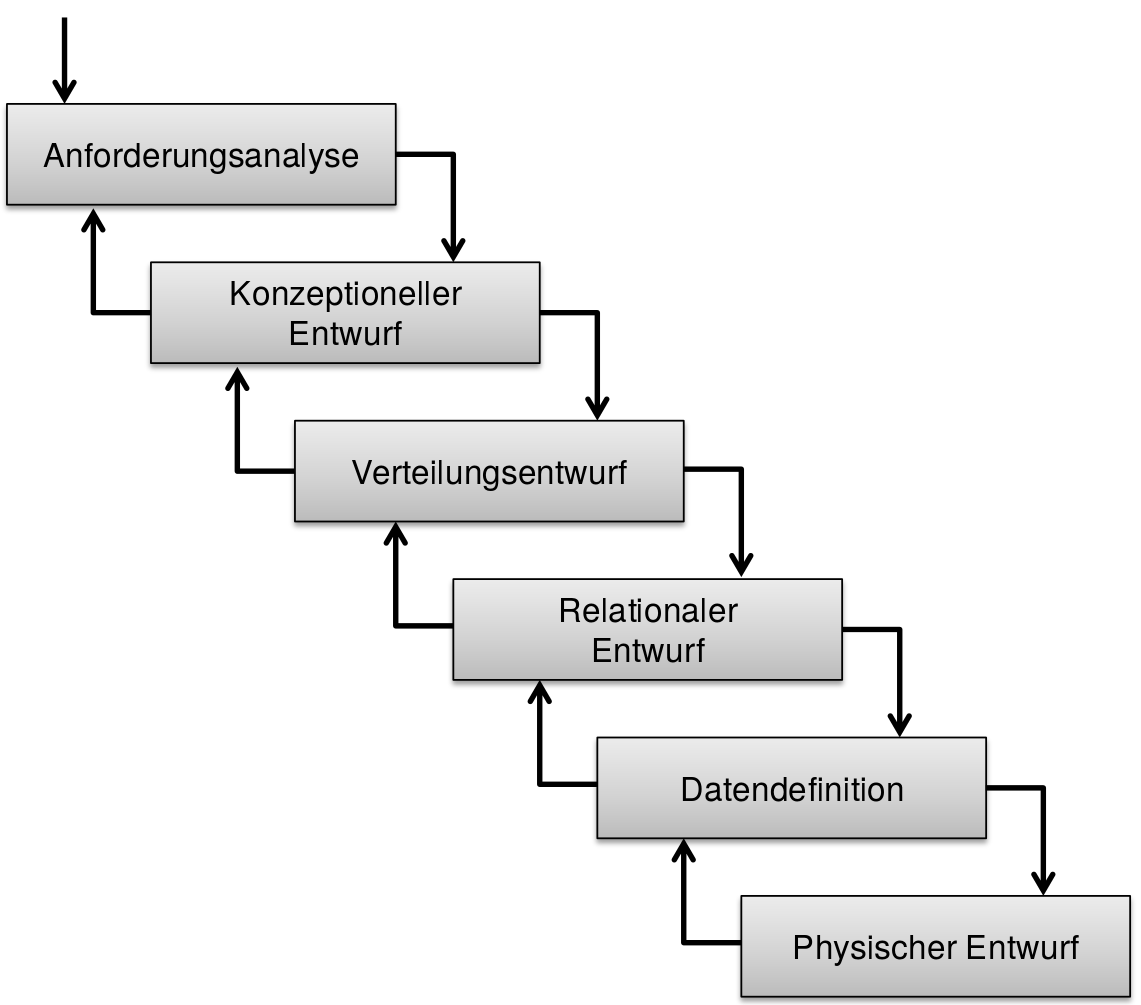
\includegraphics[width=0.33\textwidth]{Phasenmodell}\end{figure}

\textbf{Datenbankentwurf -- Modellierung}
\begin{items}
	\item Ausschnitt der Wirklichkeit mit Schema beschreiben
	\item Typen = Struktur der Entitäten
	\item Welche Konsistenzbedingungen sind sinnvoll?
	\item \underline{Schemakonsistenz}: Einhaltung der durch Schema vorgegebenen Konsistenzbedingungen (= von DBMS überprüfbar! )
\end{items}

\textbf{SQL}
\begin{items}
	\item = standardisierte Sprache für DB-Zugriff (relational)
	\item Aspekte:
	\begin{enumeration}
		\item Schemadefinition
		\item Datenmanipulation (Einfügen, Löschen, Ändern)
		\item Anfragen
	\end{enumeration}
\end{items}

\newpage

\textbf{SQL -- SQL-DDL}
\begin{items}
	\item = \emph{SQL data definition language}
	\item Teilbereich von SQL, der zu tun hat mit Definition von:
	\begin{enumeration}
		\item Typen
		\item Wertebereichen
		\item Relationsschemata
		\item Integritätsbedingungen
	\end{enumeration}
\end{items}

\textbf{SQL -- als Definitionssprache}
\begin{enumeration}
	\item Externe Ebene: 
		\begin{lstlisting}[language=sql]
{ create | drop } view;
		\end{lstlisting}
	\item Konzeptuelle Ebene:
		\begin{lstlisting}[language=sql]
{ create | alter | drop } table;
{ create | alter | drop } domain;
		\end{lstlisting}
	\item Interne Ebene:
			\begin{lstlisting}[language=sql]
{ create | alter | drop } index;
		\end{lstlisting}
\end{enumeration}

\textbf{Data Dictionary}
\begin{items}
	\item = Menge von Tabellen und Sichten
	\item Wie Datenbank aufgebaut
	\item Enthält keine Anwendungsdaten, sondern Struktur-Metadaten
\end{items}

\textbf{SQL -- Tabelle anlegen}
\begin{items}
	\item \begin{lstlisting}[language=sql]
create table Kuenstler
  (KID integer, NAME varchar(200), 
   LAND varchar(50) not null, JAHR integer, 
   primary key (KID))
\end{lstlisting}
\end{items}

\textbf{SQL -- Wertebereiche}
\begin{items}
	\item \lstinline[language=sql]{integer} (auch \lstinline[language=sql]{int})
	\item \lstinline[language=sql]{smallint}
	\item \lstinline[language=sql]{float(p)} (auch \lstinline[language=sql]{float})
	\item \lstinline[language=sql]{decimal(p,q)} (auch \lstinline[language=sql]{numeric(p,q)}, jeweils mit \lstinline[language=sql]{q} Nachkommastellen)
	\item \lstinline[language=sql]{character(n)} (auch \lstinline[language=sql]{char(n)} oder \lstinline[language=sql]{char} für \( n=1 \))
	\item \lstinline[language=sql]{character varying(n)} (auch \lstinline[language=sql]{varchar(n)}, String variabler Länge bis Maximallänge \( n \))
	\item \lstinline[language=sql]{bit(n)} (oder \lstinline[language=sql]{varying(n)} analog für Bitfolgen)
	\item \lstinline[language=sql]{date}, \lstinline[language=sql]{time}, \lstinline[language=sql]{timestamp}
\end{items}

\textbf{Wertebereiche -- Custom}
\begin{items}
	\item \begin{lstlisting}[language=sql]
create domain Gebiete varchar(20)
  default 'Informatik'
\end{lstlisting}
	\item \begin{lstlisting}[language=sql]
create table Vorlesungen
  (Bezeichnung varchar(80) not null, SWS smallint,
   Semester smallint, Studiengang Gebiete)
\end{lstlisting}
\end{items}

\textbf{Integritätsbedingungen}
\begin{items}
	\item Schlüssel kann aus mehreren Attributen bestehen
	\item \underline{Fremdschlüssel}: \begin{lstlisting}[language=sql]
create table Titel
  (TITLEID integer not null, NAME varchar(200), 
   KID integer, primary key (TITLEID), 
   foreign key (KID) references Kuenstler(KID))
\end{lstlisting}
	\item \lstinline[language=sql]{default}-Klausel: Standardwert für Attribut
	\item \lstinline[language=sql]{check}-Klausel: weitere lokale Integritätsbedingungen
	\item \begin{lstlisting}[language=sql]
create table Vorlesungen
  (Bezeichnung varchar(80) not null, SWS smallint,
   Semester smallint, check(Semester between 1 and 9), 
   Studiengang Gebiete)
\end{lstlisting}
\end{items}

\newpage

\textbf{SQL -- alter und drop}
\begin{items}
	\item \begin{lstlisting}[language=sql]
alter table Lehrstuehle
  add Budget decimal(8,2)
\end{lstlisting}
	\item \( \leadsto \) Änderung Relationsschema im Data Dictionary, existierende Daten werden um \lstinline[language=sql]{null}-Attribut erweitert
	\item \begin{lstlisting}[language=sql]
drop spaltenname { restrict | cascade }
\end{lstlisting}
\item \( \leadsto \) Attribut löschen, falls
\begin{enumeration}
	\item \lstinline[language=sql]{restrict}: keine Sichten/Integritätsbedingungen mit diesem Attribut definiert wurden
	\item \lstinline[language=sql]{cascade}: gleichzeitig diese Schichten/Integritätsbedingungen mitgelöscht werden sollen
\end{enumeration}
\item \begin{lstlisting}[language=sql]
drop table basisrelationenname { restrict | cascade }
\end{lstlisting}
\item \( \leadsto \) analog zu Attribut
\end{items}

\textbf{Speicherhierarchie}
\begin{figure}[H]\centering\label{Speicherhierarchie}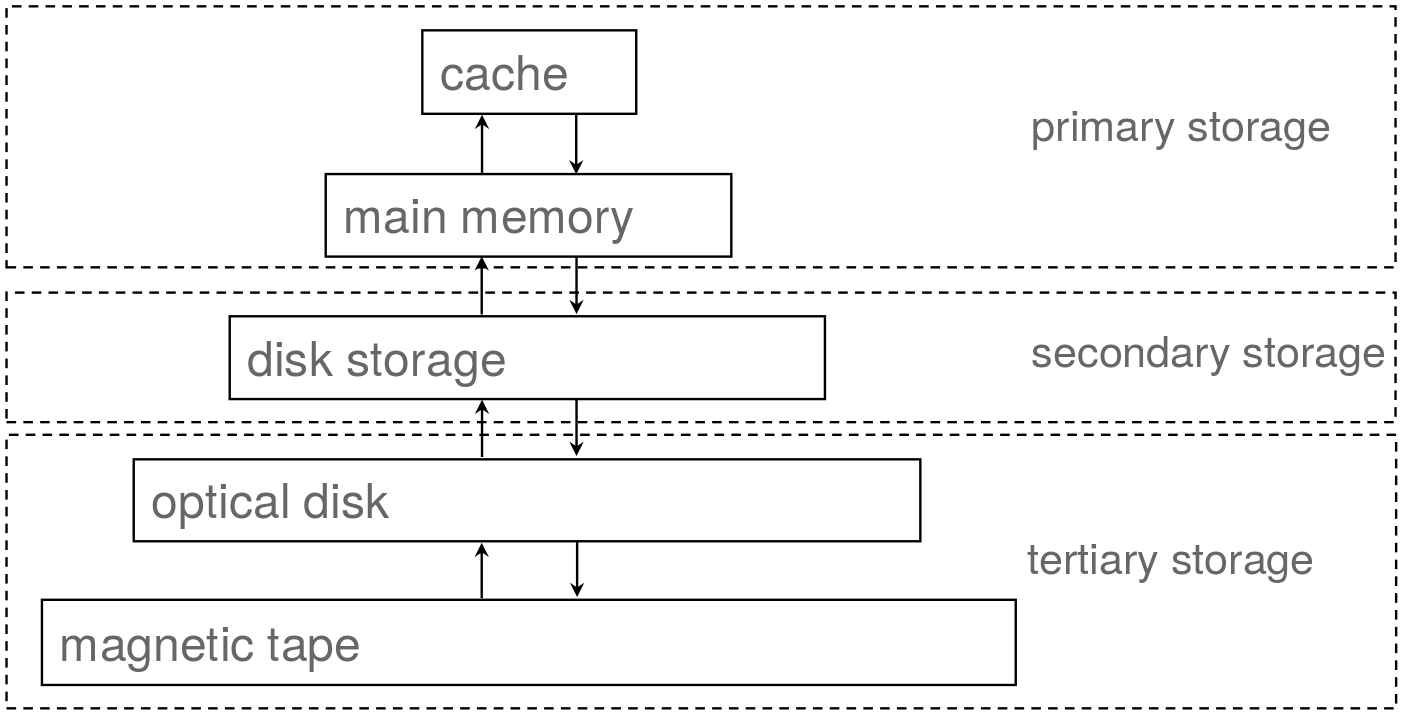
\includegraphics[width=0.33\textwidth]{Speicherhierarchie}\end{figure}

\textbf{Index}
\begin{items}
	\item Für mehrere Attribute möglich
	\item Index für (gpa, name) \( \neq \) Index für (name, gpa)
	\item Index kann nachträglich angelegt bzw. gelöscht werden, ohne Daten selbst zu löschen
	\item Index Bestandteil der physischen Ebene, Index-Definition Teil des internen Schemas
	\item \lstinline[language=sql]{select name from Student where gpa > 4} liefert Ergebnis unabhängig von Existenz eines Index -- wenn vorhanden erhebliche Beschleunigung
	\item \lstinline[language=sql]{create unique index typ on auto(hersteller, modell, baujahr)} \\* hilft bei Herstellersuche, weniger bei Suche nach Baujahr
\end{items}
\begin{figure}[H]\centering\label{Index}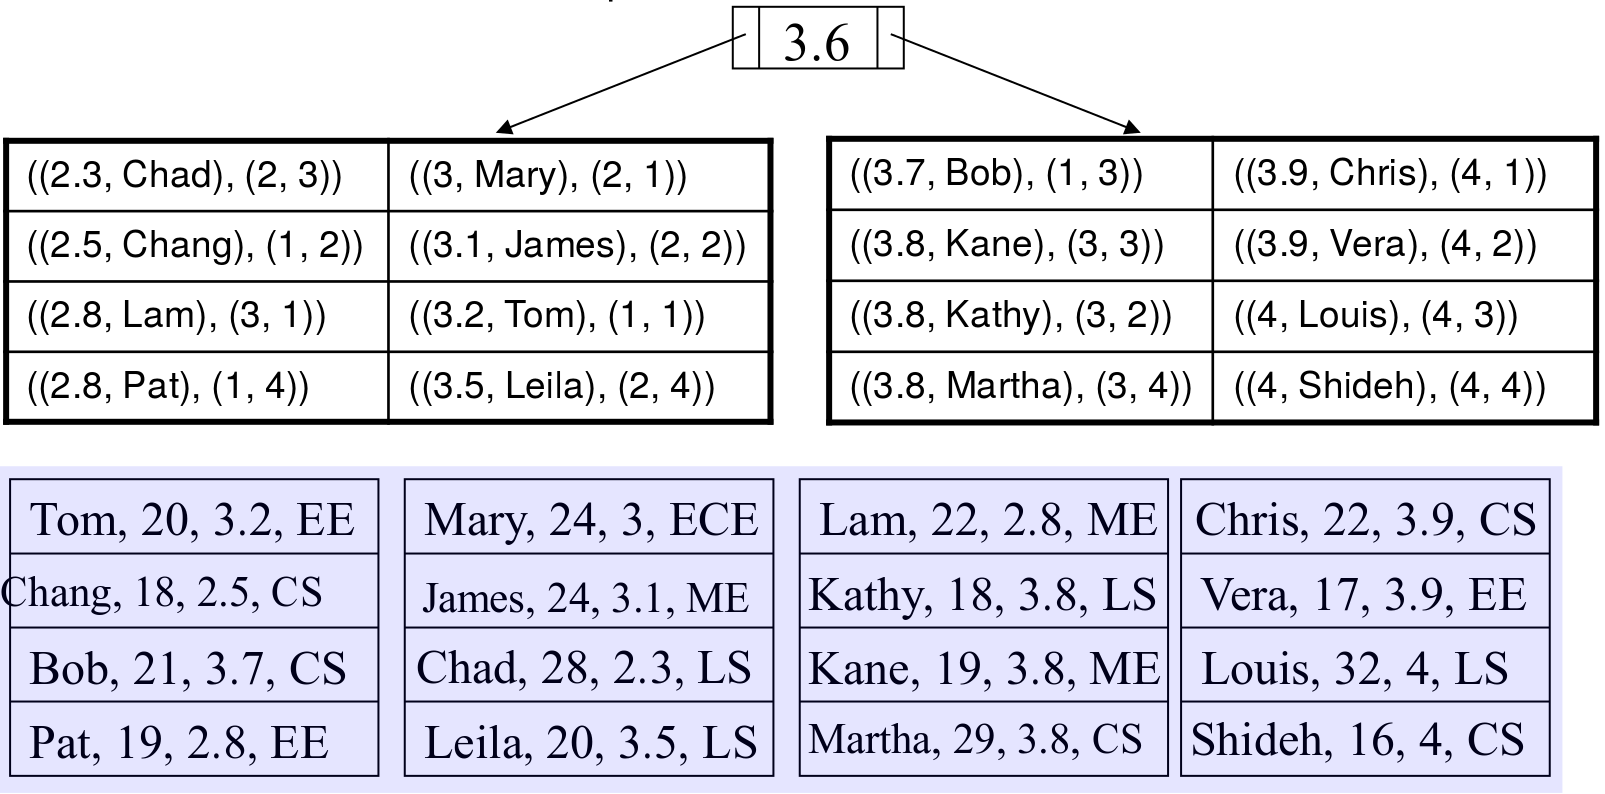
\includegraphics[width=0.33\textwidth]{Index}\end{figure}

\begin{fragen}
	\begin{enumeration}
		\item Erläutern Sie anhand eines Anwendungsbeispiels, warum man die Menge der zulässigen Zustände einschränken will.
		\item Erläutern Sie: Schema-Konsistenz, Datenbasis-Konsistenz.
		\item Was ist ein (DB-)Schema?
		\item Was ist das Data Dictionary?
		\item Warum sollte man sich die Mühe machen, Integritätsbedingungen als Teil des DB-Schemas zu formulieren?
		\item Sind Integritätsbedingungen Bestandteil des internen oder des konzeptuellen Schemas? Begründen Sie Ihre Antwort.
		\item Wieso sind Indices Bestandteil des internen und nicht des konzeptuellen Schemas?
		\item Geben Sie Beispiele dür DB-Features an, die zeigen, dass DB-Systeme physische Datenunabhängigkeit nicht vollständig umsetzen.
	\end{enumeration}
\end{fragen}